\chapter{Arhitectura platformei}
 Provocarea de a elabora o platforma web destinata atat auditorilor publici cat si reprentatilor institutiilor din administratia publica  a impus nevoie de crea o arhitectura dinamica, modulara si usor de marit in cazul adaugarii a noi functionalitati.
 
De asemenea, un numar mare de functionalitati necesita implementarea si a diferite \textit{design pattern-uri}, care se asigura ca modulule definite comunica intr-un mod cat mai eficient intre ele si promoveaza reutilizarea codului deja scris.

Acest capitol incearca sa descrie motivatia pentru alegerile facute in materie de tehnologii folosite pentru a dezvolta componentele cheie ale aplicatiei: frontend, backend stocarea datelor si cateva aspecte legate de securitatea de baza a platformei; cat si o comparatie sumara intre potentialii competetitori ai alegerilor facute.

\section {Arhitectura generala}
Arhitectura generala a fost gandita de la inceput intr-un mod care permite adaugarea de noi functionalitati in aplicatie fara a deteriora structura sau functionalitatile deja implementate.

Acestea fiind zise, proiectul este impartit in doua mari componente (client si server)  care comunica intre ele prin intermediul \textit{request-urilor HTTPS} ,si anume:

\begin{itemize}
	
	\item componenta de server, este alcatuita din diferite \textit{endpoint-uri}  Web API care ofera functionalitati clientilor sai, aceasta comunicand si cu mediul de stocare al datelor, o baza de date MySQL;
	
	\item componenta client, sau interfata grafica a platformei, este o aplicatie web interactiva de tipul SPA (\textit{Single page application}), oferind functionalitatile descrise prin intermediul \textit{request-urilor} catre server, urmand ca mai apoi sa fie afisate pe pagina web prin intermediul \textit{WebAssembly}.
\end{itemize}  

\subsection*{Diagrame de context C4 }

Diagramele de context C4 reprezinta un stadard in ceea ce priveste o vedere de ansamblu, dar care merge inspectata in detaliu pentru fiecare component al aplicatiei, astfel promovand o ierarhizarea si o intelegere a intreg sistemului mai buna.\\


\subsection*{Nivelul 1}
Primnul nivel al diagramelor de context ofera o viziune de ansamblu asupra sistemelor ce compun solutia descrisa.
\vspace{1cm}
\begin{figure}[h]
	\centering
	
	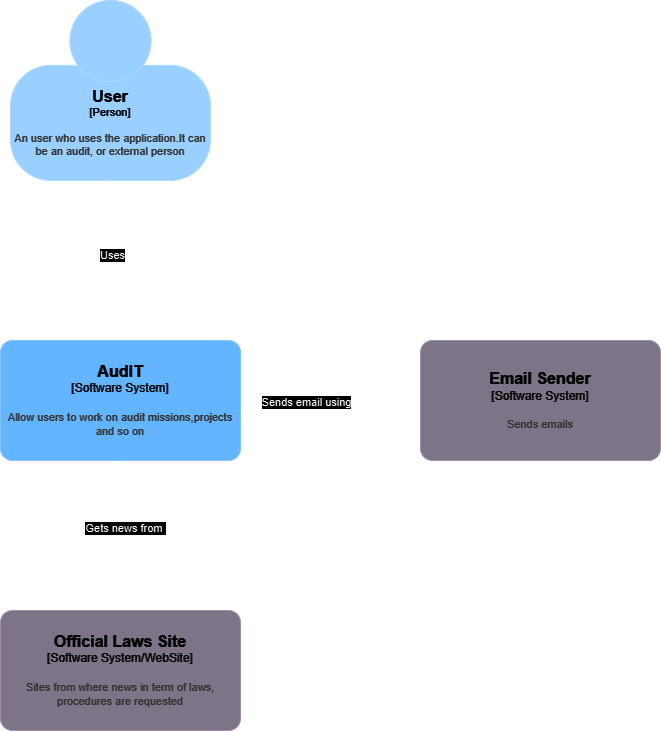
\includegraphics[width=0.6\textwidth]{c2/C4_level1}
	\caption{Primul nivel diagrama C4}
\end{figure}

\newpage
\subsection*{Nivelul 2}
Al doilea nivel prezinta \textit{containerele} principale ale fiecaurui sistem din nivelul anterior, astfel oferind o viziune mai clara asupra arhitecturii generale a platformei si a functionalitatilor sale.
\vspace{1cm}
\begin{figure}[h]
	\centering
	
	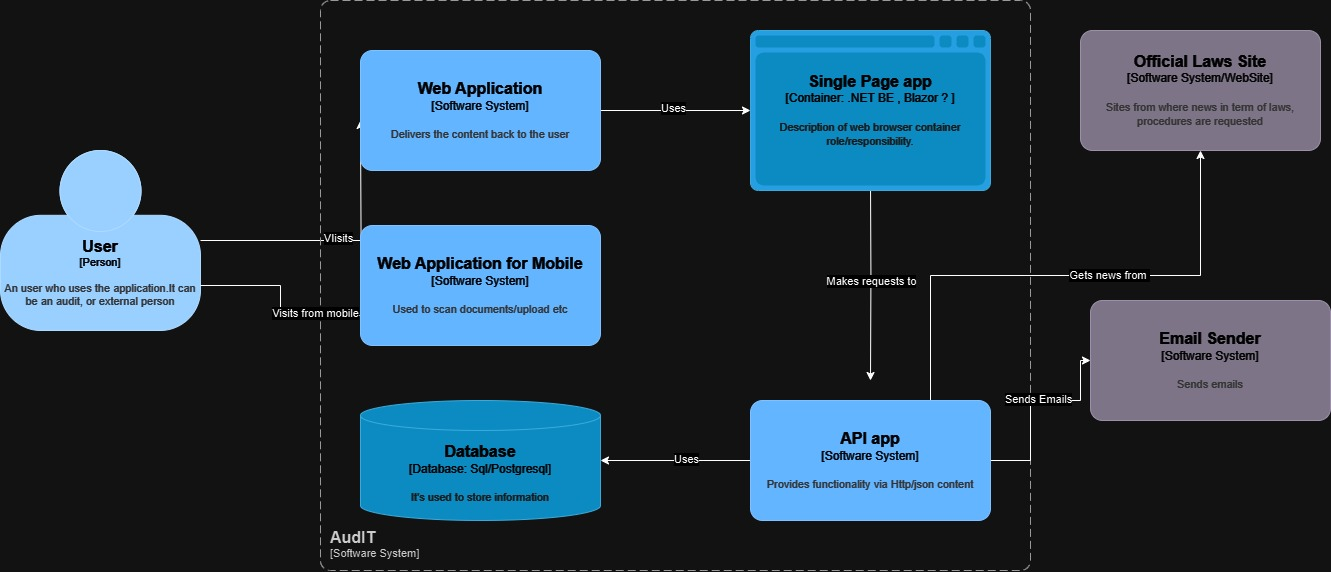
\includegraphics[width=0.7\textwidth]{c2/C4_level2}
	\caption{Al doile nivel din diagrama C4}
\end{figure}

\subsection*{Nivelul 3}
Al treilea nivel ofera o viziune mult mai detaliata asupra componentelor ce apartin \textit{container-ului} de la nivelul secund, oferind abstractii cat mai apropiate de codul ce urmeaza a fi scris pentru a le implementa.

\vspace{1cm}
\begin{figure}[h]
	\centering
	
	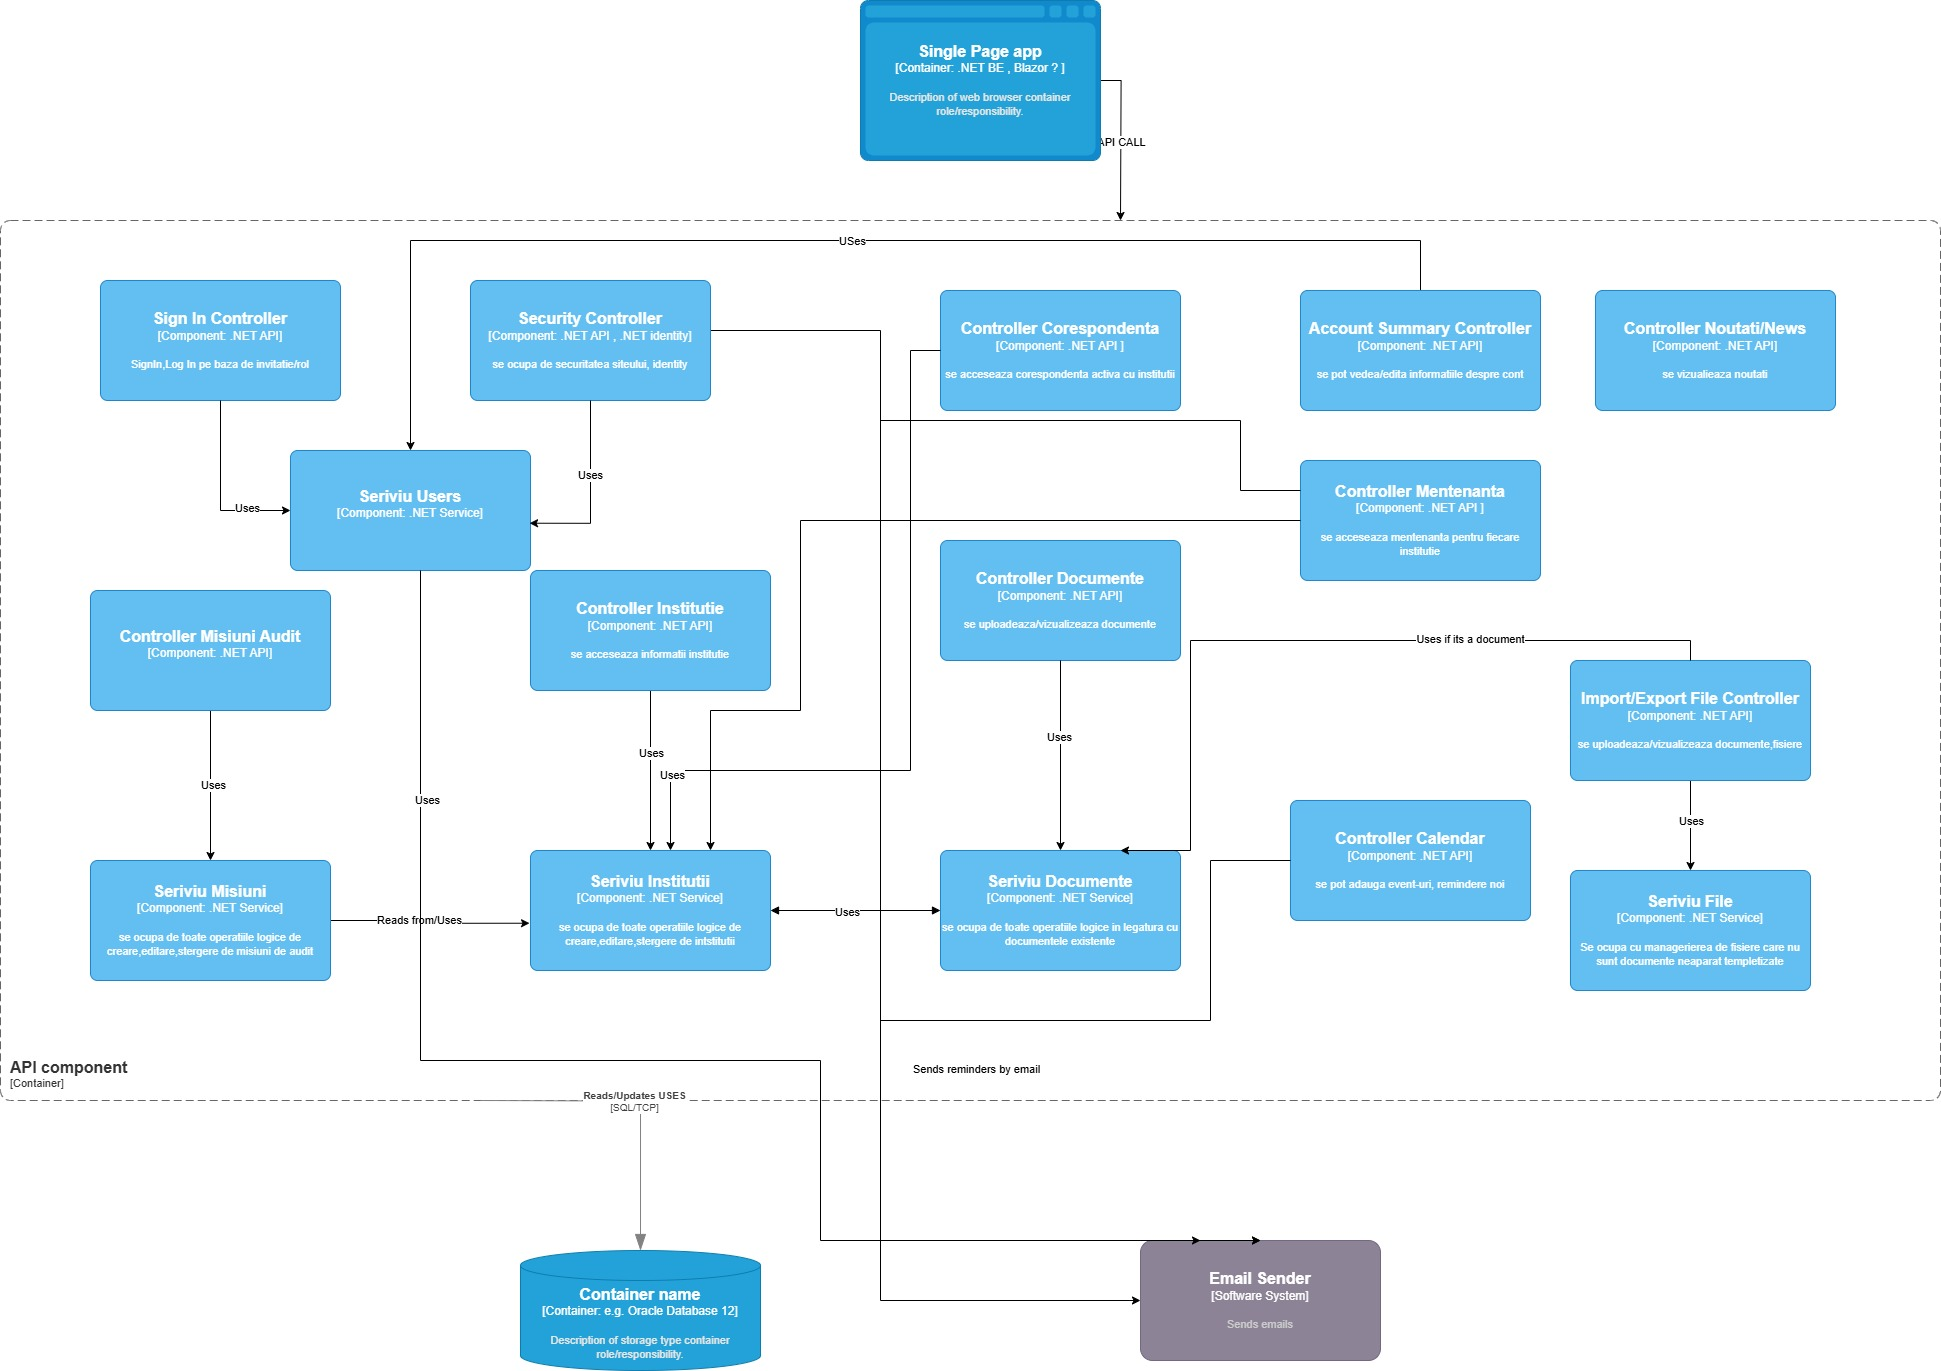
\includegraphics[width=1\textwidth]{c2/C4_level3}
	\caption{Nivelul trei din diagrama C4}
\end{figure}



\section{Arhitectura serverului}

\subsection*{Arhitectura \textit{monolith}}

Arhitectura generala a serverului este una de tip \textit{monolith} traditional, impartita pe module, cu dependente slabe intre ele, care comunica intre prin intermediul unor contracte (interfete) bine definte.\\
Alegerea acestui tip de arhitectura a fost motivata de mai multe avantaje cheie ale acesteia: 
\begin{itemize}
	\item simplitatea dezvoltarii in cadrul arhitecturii de tip monolith permite lucrul pe o singura baza de cod , ceea ce simplica major procesul de dezvoltare, testare si de depistare a erorilor, fiind esentiala in fazele de inceput al unui proiect;
	
	\item  performanta sporita in cadrul unui aplicatii care raspunde \textit{request-urilor}, astfel un singur \textit{API} poate raspunde la toate cererile, eliminand nevoia de a activa si alte \textit{API-uri} externe pentru indeplinirea sarcinii, ca in cazul arhitecturii de micro-servicii;
	
	\item usurinta testarii de tip \textit{unit-testing} cat si \textit{integration-testing} intrucat toate modulele sunt in acelasi loc;
	
	\item  depistarea erorilor si rezolvarea lor este mult mai rapida.
\end{itemize}
Conform oricare alegeri, trebuie puse in balanta avantajele si dezavantajele pe care aceasta le ofera si  sa se compare strict cu nevoile si problemele care se incearca a rezolva. Privind in ansamblu si pe termen lung, arhitectura de tip \textit{monolith} prezinta si unele dezavantaje: 

\begin{itemize}

 \item dezvoltarea incetinita in momentul in care functionalitatile pe care dorim sa le implementam cresc ca si numar, intrucat toate modulele sunt comasate intr-un singur loc;
 
 \item \textit{scalabilitate redusa} datorita stransei legaturi dintre componentele prezente in aplicatie;
 
 \item 	orice schimbare adusa in materie de noi functionalitati necesita lansarii intregii aplicatii, nu doar a unui singur modul.

\end{itemize}

Pentru a diminua efectele negative pe care aceste dezavantaje le au asupra intregului proces de dezvoltare a aplicatiei, am incercat implementarea diferitelor solutii in materie de arhitectura, \textit{desing pattern-uri} cretionale, arhitecturale cat si a numeroase practici bune comune in scrierea si mentenanta codului.

\subsection*{Arhitectura \textit{Clean Code}}
Arhitectura \textit{Clean Code } este bazata pe ideea principala precum ca stratul de logica interna (\textit{business layer}) este situat central in diagrama circulara, astfel acesta este protejat de schimbari externe. Aceasta proprietate poate fi reformulata astfel incat se defineste \textbf{Regula Dependentei} care presupune ca dependintele pot sa fie orientate doar inspre interiorul cercului, astfel niciunul din modulele interioare nu ar trebui sa fie legat in orice fel de un modul exterior acestuia.

\begin{figure}[h]
	\centering
	
	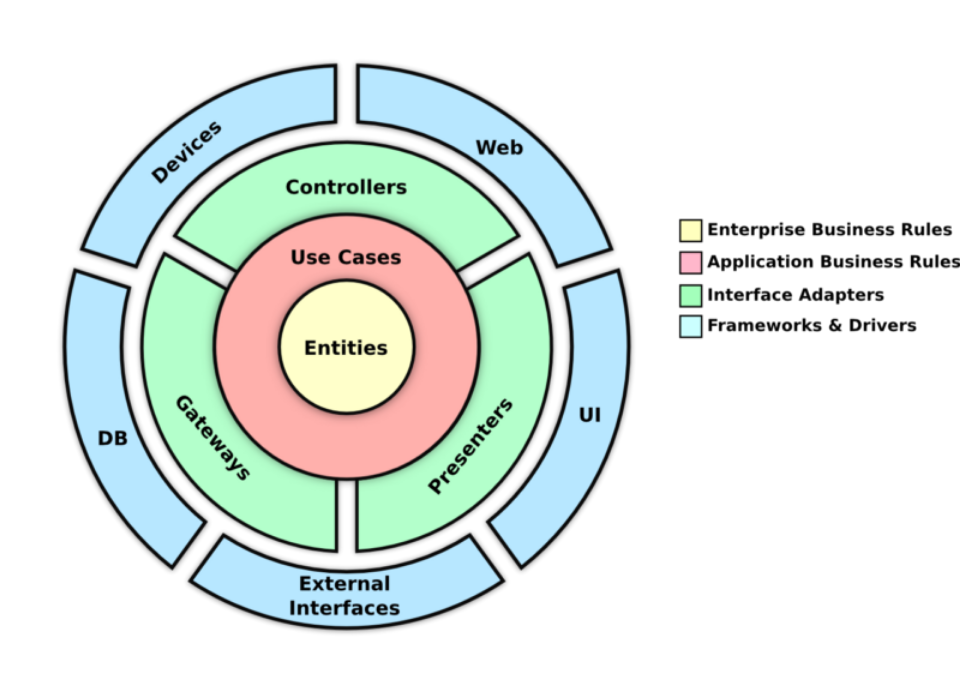
\includegraphics[width=0.6\textwidth]{c2/clean_architecture.png}
	\caption{Structura arhitecturii \textit{Clean code}}
\end{figure}

Adoptarea acestui tip de arhitectura impreuna cu cea de tip \textit{monolith} include mai multe beneficii cum ar fi:

\begin{itemize}

	\item mentenanta sporita datorata faptului ca modulele sau straturile principale ale aplicatiei si logica ce le faciliteaza comnunicarea eficienta sunt separate, incurajand astfel si o intelegere mai detaliata si simplificata a intregului sistem;
	
	\item flexibilitate din punct de vedere al schimbarii tehnologiilor exterioare, stratul de logica interna este independent de ceea ce se intampla in exteriorul sau;
	
	\item testarea componentelor se poate face atat individual cat si in relatie cu alte module, astfel eliminand nevoia de testare a intregii aplicatii;
	
	\item stratul de logica interna este independent de baza de date folosita, asftel serverul de stocare al datelor poate fi schimbat cu usurinta.

\end{itemize} 
Modul in care arhitectura de tip \textit{Clean Code} a fost implementata in aceste proiect consta in separarea straturilor aplicatiei, astfel incat avem:

\begin{itemize}
	\item  \textit{Core Layer} fiind structura principala ce confera logica interna a aplicatiei.Acesta cuprinde \textit{Domain} unde sunt modelate entitatile aplicatiei respectiv \textit{Application} unde este definita toata logica interna a serverului,
	de la declaratiile abstracte ale interfetelor la definerea serviciilor proprii de care se vol folosi ulterior straturile externe ale arhitecturii;
	
	\item \textit{API Layer} este partea structurala care defineste \textit{endpoint-urile} aplicatiei prin diferite \textit{controllere}, expunand astfel functionalitatile aplicatiei la internet;
	
  	\item \textit{UI Layer} defineste structura de prezentare a aplicatiei si este formata din parte de \textit{Frontend} a aplicatiei;
  
 	 \item \textit{Infrastructure Layer} in care gasim logica ce se ocupa de comunicarea cu serviciile externe cum ar fi baza de date, AWS sau servicii de identitate.
 	 
\end{itemize}

\subsection*{\textit{Design pattern-uri} utilizate}

\textit{Design pattern-urile}, potrivit definitiei, sunt solutii generale si reutilizabile asupra problemelor comune ce pot aparea in decursul dezvoltarii unei aplicatii software.\\
Utilizare lor conduce la o buna mentananta a codului scris, posbilitatea de a reutiliza module deja scrise, imbunatateste comunicare si legaturile dintre module si incurajeaza un stil de cod cat mai elegant si usor de inteles.\\
In implementarea aplicatiei au fost folosite \textit{desing pattern-uri} din diferite categorii astfel incat in aceasta subsectiune se vor discuta cateva exemple utilizate.

\subsection*{\textit{Optional pattern}}
Acesta este un model de proiectare care ajuta la gestionarea valorilor care pot sau nu fi prezente, astfel avand valoarea \textit{null}. \textit{Pattern-ul} se asigura ca este eliminata valoarea \textit{null}, care de cele mai multe ori este o sursa comuna in erori la rularea codului (\textit{runtime}).

Solutia prezentata de acest model este crearea unei clase \textit{template} care incapsuleaza valoarea propriu zisa a entitatii pe care o construim. Spre exemplu, in cazul in care vrem sa cream o noua entitate de tipul \textit{User} dar la \textit{runtime} apare o eroare, executia programului nu se va opri, iar valoarea entitatii va fi incapsulata intr-un tip   \textit{Result\textless User\textgreater}

 cu parametrul \textit{Succes} setat pe fals, indicand astfel ca procesul de creare a esuat.\\

\begin{figure}[h]
	\centering
	
	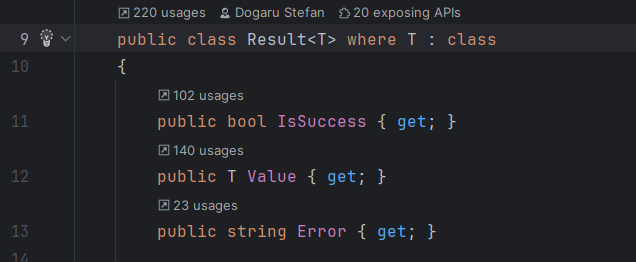
\includegraphics[width=0.8\textwidth]{c2/optional_patterns}
	\caption{Exemplu de clasa care implementeaza Optional Pattern}
\end{figure}

\subsection*{\textit{Mediator pattern}}
Acest \textit{design pattern} este unul de tip comportamental si se asigura ca nu exista dependente haotice intre entitatile/clasele din codul scris. Modelul restrictioneaza comunicarea directa intre obiecte si le obliga sa interactioneaze doar prin intermediul unui \textit{mediator}.

Acest model este implementat prin utilizarea unei interfate sau clase abstracte care stie toate referintele la componentele care vor sa comunice. In acest mod, in loc sa trimita solicitari directe, un obiect comunica prin intermediul mediatorului, acesta stiind unde sa redirectioneaze cererea primita.


\begin{figure}[h]
	\centering
	
	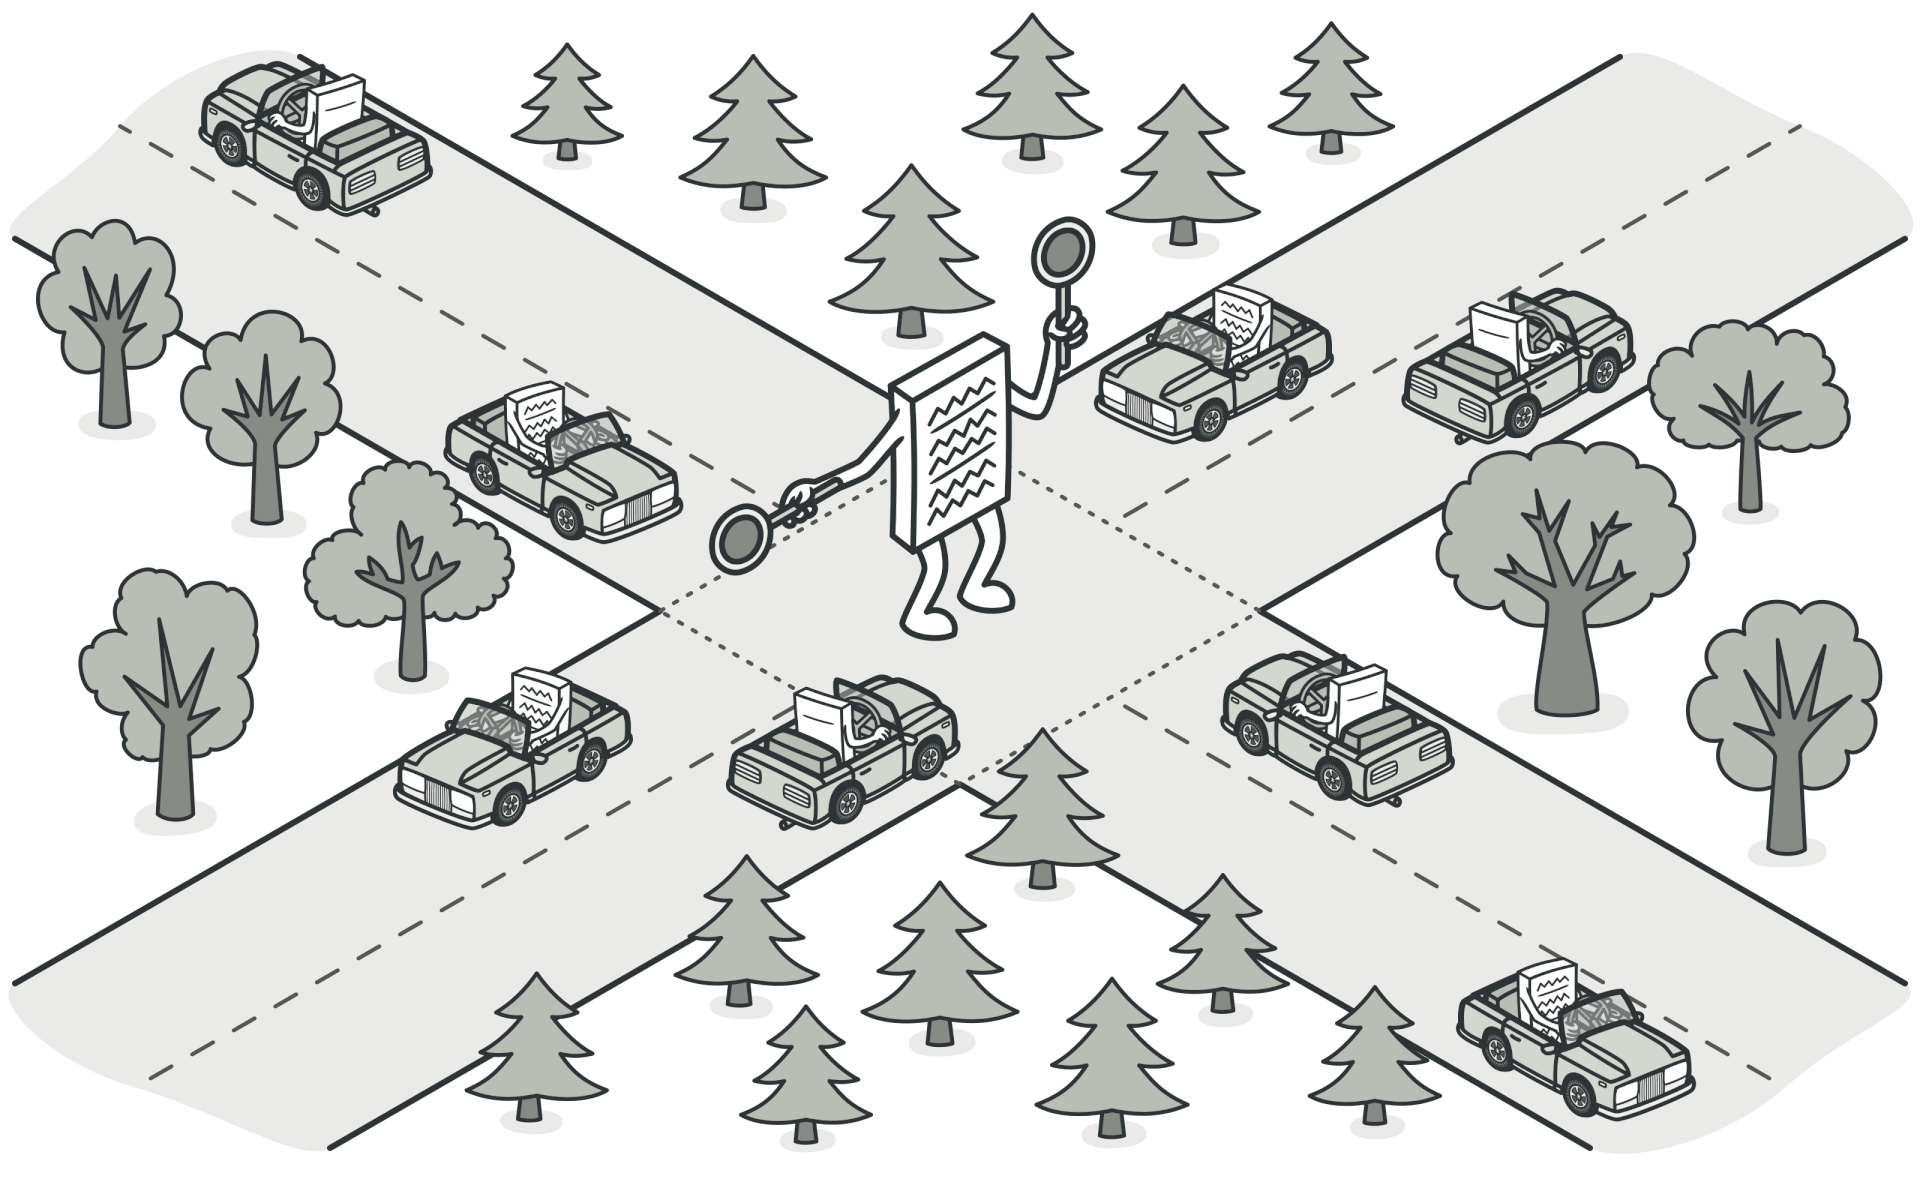
\includegraphics[width=0.6\textwidth]{c2/mediator_pattern}
	\caption{Ilustratie \textit{mediator pattern}}
\end{figure}

	\newpage
\subsection*{\textit{Command pattern}}	

Acest \textit{design pattern} este de asemenea unul de tip comportamental si se utilizeaza partial de \textit{design pattern-ul Mediator}, transformand astfel o comanda, spre exemplu o cerere de creare a unei noi entitati, intr-un obiect independent, acesta ulterior fiind trimis catre mediator si executat in \textit{handler-ul} corespunzator acestuia, de obicei numit \textit{receiver}.

In contextul dezvoltarii partii de server a aplicatiei AudIT, acesta este utiliat, impreuna cu modelul Mediator pentru a delega orice comanda (\textit{request}) primita catre obiectul care stie sa o execute. In acest mod, se elimina dependente stranse intre obiecte, promovand un cod cat mai bine organizat si elegant.\\

\vspace{1cm}
\begin{figure}[h]
	\centering
	
	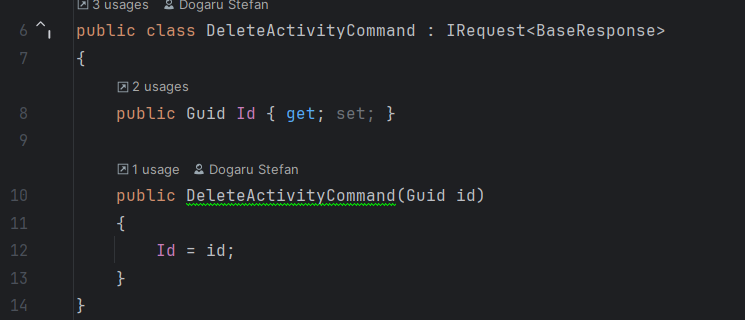
\includegraphics[width=0.7\textwidth]{c2/command_pattern1}
	\caption{Exemplu clasa de tip \textit{Command}}
\end{figure}



\vspace{1cm}
\begin{figure}[h]
	\centering
	
	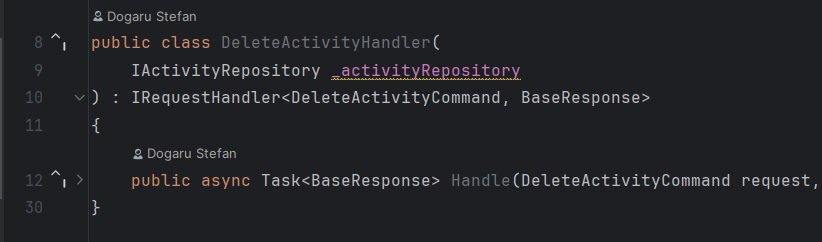
\includegraphics[width=0.7\textwidth]{c2/command_pattern2}
	\caption{Exemplu clasa de tip \textit{Handler/Receiver}}
\end{figure}


\subsection*{\textit{Repository pattern}}

Folosit in special in dezvoltarea aplicatiilor web, acest \textit{design pattern} separa logica interna a aplicatiei de accesul direct la date (baza de date). Acesta se utilizeaza de interfate pentru a crea un strat separator intre declararea abstracta a acestor constracte si implementarea concreta a functiilor care acceseaza datele la nivel de baza.

Prin acest model, comunicarea dintre module se realizeaza prin intermediul contractului foarte bine stabilit, astfel eliminand posibilitatea ca un modul abstract sa acceseze direct un modul de acces de date.\\


\vspace{1cm}
\begin{figure}[h]
	\centering
	
	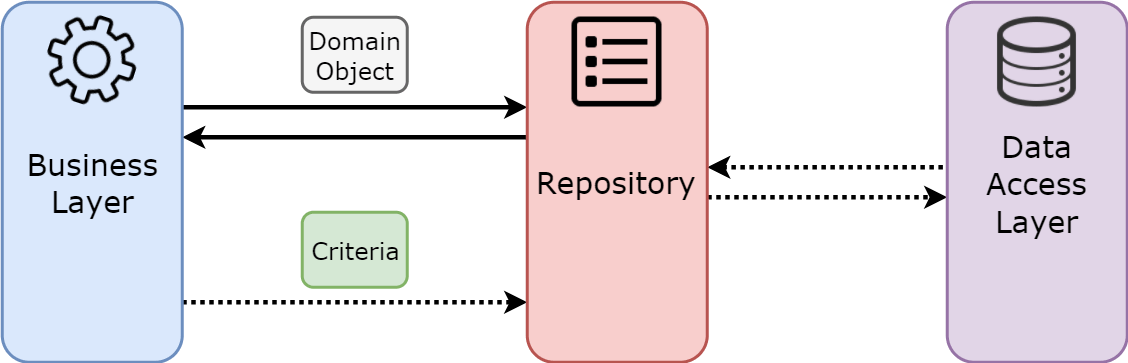
\includegraphics[width=0.8\textwidth]{c2/repository_pattern}
	\caption{Diagrama \textit{repository pattern}}
\end{figure}
\subsection*{Descriere \textit{endpoint-uri} utilizare}
\textit{Endpoint-urile} sunt componentele de baza ale comunicarii aplicatiilor prin intermediul internetului si a \textit{API-urilor}. Partea de server expune informatii si facilitati clientilor prin intermediul acestor \textit{endpoint-uri}, astfel acestia avand posiblitatea de a comunica prin intermediul acestor puncte cu aplicatia si cu logica interna a acesteia.

\textit{Endpoint-urile} create de server sunt organizate conform fiecarei entitati din \textit{Domeniul} aplicatiei , pentru o mai buna navigare si intelgere a structurii in ansamblu, cat si avand in vedere actiunea pe care clientul doreste sa o realizeze.

Principalele \textit{endpoint-uri} expuse clientilor pe partea de server sunt :

\begin{itemize}
	
	\item \textit{endpoint-urile} care gestioneaza actiunile utilizatorului legate de autentificare: inregistrare, autentificare, iesire din cont, verificare email cat si actualizare a informatiilor contului de utilizator.Aceste \textit{endpoint-uri} sunt centrate in jurul entitatii de Utilizator;
	
	\item \textit{endpoint-urile} care se ocupa de logica gestionarii entitatilor de tip Misiune de audit, astfel permitand crearea, listarea, stergerea acestora cat si actualizarea informatiilor si obtinerea de informatii partajate cu alte entitati;
	
	\item \textit{endpoint-urile} care gestioneaza obiectivele unei misiuni de audit;
	
	\item \textit{endpoint-urile} care trateaza actiunile unui obiectiv respectiv riscurile acestuia;
	
	\item \textit{endpoint-urile} care administreaza actiunile referitoare la entitatile de tip Recomandare;
	
	\item punct de accees asupra entitatilor de tip Document, existand posibilitatea de a crea, a incarca, descarca si a sterge documente salvate pe platforma;
	
	\item \textit{endpoint-urile} care gestioneaza actiunile de export de date si de autocompletare a unor documente de tip sablon cu date de pe platforma;
	
	\item \textit{endpoint-urile} care permit configurarea institutiilor si a departamentelor de pe platforma.
	
\end{itemize} 

De asemenea, \textit{server-ul} expune prin intermediul altor \textit{ endpoint-uri} functionalitati cum ar fi configurarea accesului la resurse partajate, gestionarea activitatilor desfasurate pe platforma cat si un sistem de notificari ce permite actualizarea informatiilor disponibile pe aplicatie in timp real.


	
 

\subsection*{Tehnologii utilizate}
In dezvoltarea partii de server s-a utilizat \textit{framework-ul } ASP.NET Core impreuna cu limbajul C\#.\\
Alegerea facuta se bazeaza pe faptul ca \textit{framework-ul} este unul de tip \textit{open-source}, dezvoltat in principal de Microsoft, un actor important pe piata actuala IT,\textit{framework-ul} oferind functionalitati robuste si eficiente pentru dezvoltarea aplicatiilor web, acestea putand fi rulate pe Windows, Linux cat si MacOS.

De asemenea, C\# este un limbaj de programare multi-paradigma \textit{high-end} matur, care ofera diverse functionalitati si solutii foarte bine puse la punct atat din punct de vedere al eficientei cat si al sustenabilitatii codului.

Mai mult de atat, integrarea celor doua tehnologii cu alte servicii Microsoft este una foarte usor de realizat, acest lucru aducand un motiv in plus in alegerea facuta, pe langa ecosistemul bogat din care acestea fac parte, oferind suport pentru o gama larga de biblioteci si unelte deja integrate in functionalitatile limbajului si a \textit{framework-ului}.

In plus, s-au utilizat diferite biblioteci pentru dezvoltarea anumitor servicii, cum ar fi :
\begin{itemize}
	\item  AWSSDK.Core pentru integrarea serviciilor AWS de trimiterea a unui email sau de stocare a datelor si a fisierelor in S3 Bucket;
	
	\item  MediatR care ofera functionalitatile \textit{design pattern-ului} Mediator;
	
	\item ASP.NET Identity, serviciu pentru integrarea functionalitatilor de autentificare si autorizare in aplicatie, facilitand accesul si autorizarea utilizatorilor pe platforma;
	
	
	\item AutoMapper este o bibilioteca externa utilizata pentru a transforma diferitele tipuri de obiecte intre ele, eliminand astfel codul \textit{boilerplate} necesar pentru a copia datele de la  o entitate la alta;
	
	\item OpenXML este o biblioteca \textit{open-source} care permite manipularea fisierelor Office de tipul .XLSX sau .DOCS. Este integrata pentru a oferi utilizatorilor functionalitatea de a putea edita sau exporta pe platforma documente oficiale tip sablon.
	
\end{itemize}
   

\section{Arhitectura interfatei grafice}
Interfata grafica dezvoltata in acest proiect este realizata in \textit{framework-ul} .NET Blazor, mai exact o aplicatie de tipul \textit{WASM (Web Assembly)} care ruleaza in \textit{browser-ul} utilizatorului. Alegerea a fost facuta intrucat acest nou model arhitectural permite rularea codului direct in \textit{browser}, nemaifiind nevoie de librarii sau extensii suplimentare necesare.\\

\newpage
\subsection*{Web assembly} 
Cum ne putem da seama si din numele pe care aceasta tehnologie o poarta, este vorba despre \textit{byte-code} (cod-masina) care este executat de o componenta separata din \textit{browser} ,numita \textit{Wasm engine}.

\textit{Wasm} nu este un limbaj, ci mai degraba produsul compilarii codului scris intr-un limbaj de programare in cod-masina executabil. Majoritatea limbajelor de programare moderne  suporta compilarea codului direct intr-un fisier  binar de tip .wasm . Dupa o compilare cu succes, fisierele binare .wasm sunt incarcate in \textit{browser} cu ajutorul Javascript, urmand sa fie executate de catre componenta mentionata intr-o instanta virtuala izolata si securizata.\\

\vspace{1cm}
\begin{figure}[h]
	\centering
	
	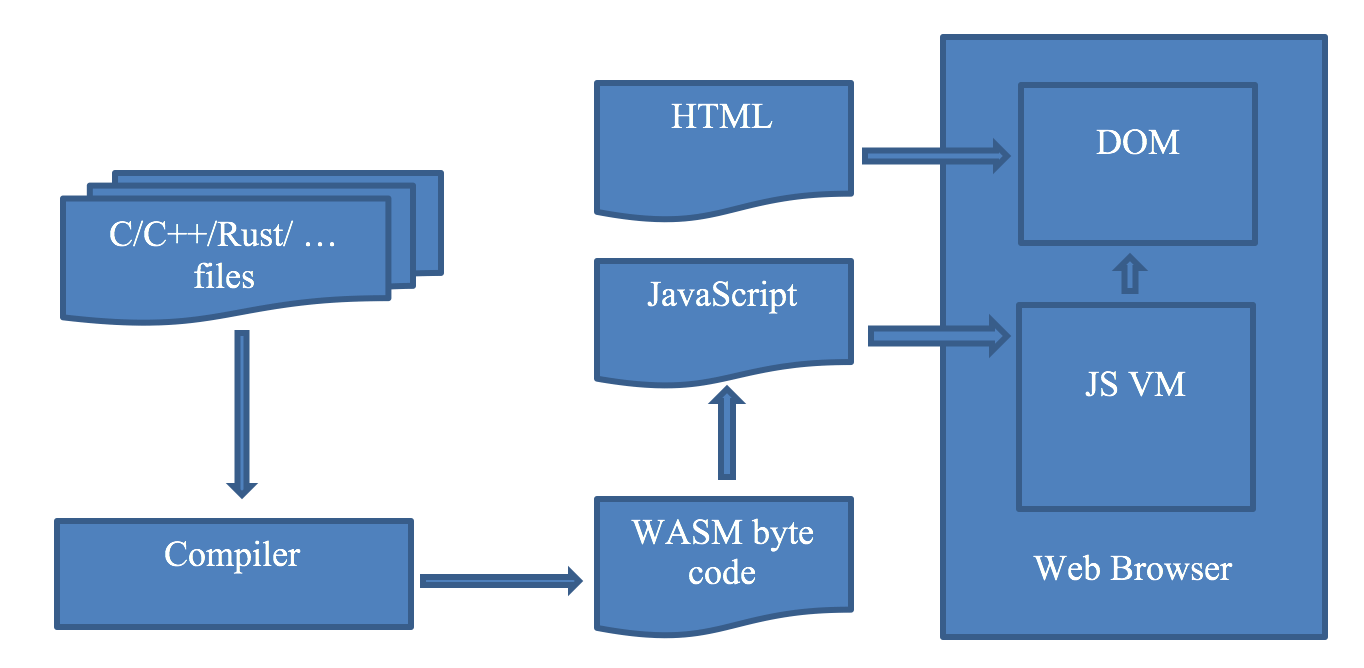
\includegraphics[width=0.7\textwidth]{c2/wasm}
	\caption{Diagrama mod functionare \textit{Web Assembly}}
\end{figure}

Un avantaj cheie al utilizarii acestei tehnologii il constituie viteza si eficienta de care da dovada. Codul ruleaza cat se poate de aproape de limitarile \textit{hardware} ale computer-ului, astfel rezultand in performante crescute si un nivel al utilizarii memoriei mai mic.\\
Pe de alta parte, exista si dezavantaje in utilizarea acestuia, intrucat momentan nu este implementat un sistem de \textit{garbage collector} care sa elimine din memorie functiile si instantele care nu mai sunt folosite in firul executiei.

\subsection*{.NET Blazor}
Pentru dezvoltarea paginilor web, s-a utilizat tehnologia .NET Blazor, un \textit{framework} relativ nou aparut, dar care promite performante crescute alaturi de un mediu de lucru bine pus la punct si eficient din punct de vedere al productivitatii dezvolarii interfatelor interactive si bogate.\\
Paginile web create in acest mod combina codul C\# cu HTML pentru a crea componente reutilizabile ce sunt  afisate si actualizate in DOM-ul virtual din \textit{browser}.\\

\vspace{1cm}
\begin{figure}[h]
	\centering
	
	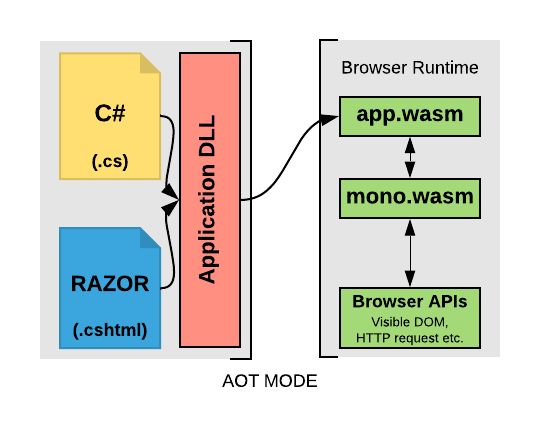
\includegraphics[width=0.7\textwidth]{c2/blazor}
	\caption{Diagrama mod functionare \textit{Blazor WebAssembly}}
\end{figure}

O functionalitate foarte importanta pe care o ofera, este utilizarea asa ziselor componente, parti fundamentale care impreuna alcatuiesc pagina web afisata utilizatorului. O componenta poate fi vazuta ca o piesa esentiala de puzzle care contribuie la afisarea finala a unei pagini web, piesa de puzzle care la randul sau poate fi creata din mai multe astfel de componente, si asa mai departe.

Un avantaj pe care Blazor il ofera dezvoltatorilor este acela ca elimina pe cat posibil utilizarea de functii si \textit{script-uri }JavaScript in crearea paginilor web. Blazor se foloseste de cod scris in C\# impreuna cu HTML si CSS pentru a elabora pagini si componente web interactive si fluide.\\

\subsection*{Radzen Components}
De asemenea, pentru o stilizare si o reutilizare a componentelor, s-a folosit libraria Radzen Components pentru a folosi controale si componente cum ar fi : tabele, butoane stilizate, teme grafice de inalta calitate, \textit{form-uri} si multe altele.\\
 Libraria Radzen Components este una de tip \textit{open-source} si ofera suport dedicat din partea comunitatii active, impreuna cu documentatie detaliata asupra tuturor functionalitatilor oferite.


\section{Stocarea datelor}

 \subsection*{Baza de date MySQL}
	MySQL este un sistem de gestionare a bazelor de date relationare open-source si reprezinta alegerea pentru care am optat a fi folosita pentru stocarea datelor in acest proiect.Acest sistem este una dintre cele mai populare solutii cand vine vorba de stocare intr-un mod relational al datelor, astfel incat acesta ofera diferite beneficii: 
	\begin{itemize}
		
		\item simplitatea cand vine vorba de utilizarea acestuia, folosindu-se de un dialect comun in interogarile sale, este foate usor de utilizat;
		
		\item securitatea datelor oferita de MySQL prin integrarea unui sistem solid de privilegii si de restrictionarea a accesului bazat pe roluri;
		
		\item flexibilitatea si functionalitatile pe care acesta le ofera sporesc productivitatea dezvoltarii aplicatiilor.
	\end{itemize} 
 
 \subsection*{Entity Framework Core}
Entity Framework Core este o tehnologie dezvoltata de Microsoft in cadrul \textit{framework-ului} .NET Core care permite dezvoltatorilor sa interactioneze cu entitatile si tabelele din baza de date prin intermediul obiectelor, eliminand astfel necesitatea de a scrie interogari clasice pentru a comunica facil cu baza de date si cu obiectele sale.

Aceasta tehnologie dispune de o serie de caracteristici si functionalitati care o fac o alegere cruciala in ceea ce priveste comunicarea intr-un mod eficient cu baza de date:
\begin{itemize}
	
	\item sistemul de \textit{migratii} similar unui \textit{version-control} al versiunii bazei de date si a relatiilor acesteia, permite dezvoltatorilor sa tina evidenta versiunii bazei de date, eventual existand posibilitatea in cazul unor erori sa se intoarca la ultima versiune stabila;
	
	\item \textit{code-first} este functionalitatea ce permite actualizarea modelului din baza de date pe baza schimbarilor din codul scris si a modificarilor din entitatile declare in codul sursa;
	
	\item suportul pentru majoritatea bazelor de date existente in momentul de fata, primind constant actualizari;
	
	\item performanta interogarilor, astfel incat sistemul este optimizat sa colecteze intr-un mod eficient rezultatele interogarilor.
	 
\end{itemize}

\subsection*{Structura bazei de date}

Pentru autentificare si autorizarea activitatilor utilizatorilor, se utilizeaza biblioteca .NET Identity Core, care pune la dispozitia dezvoltatorilor o solutie deja implementata in materie de tabele si a relatiilor dintre ele, astfel incat dezvoltatorul sa se ocupe doar de logica utilizarii acestora.
 
\vspace{1cm}
\begin{figure}[h]
	\centering
	
	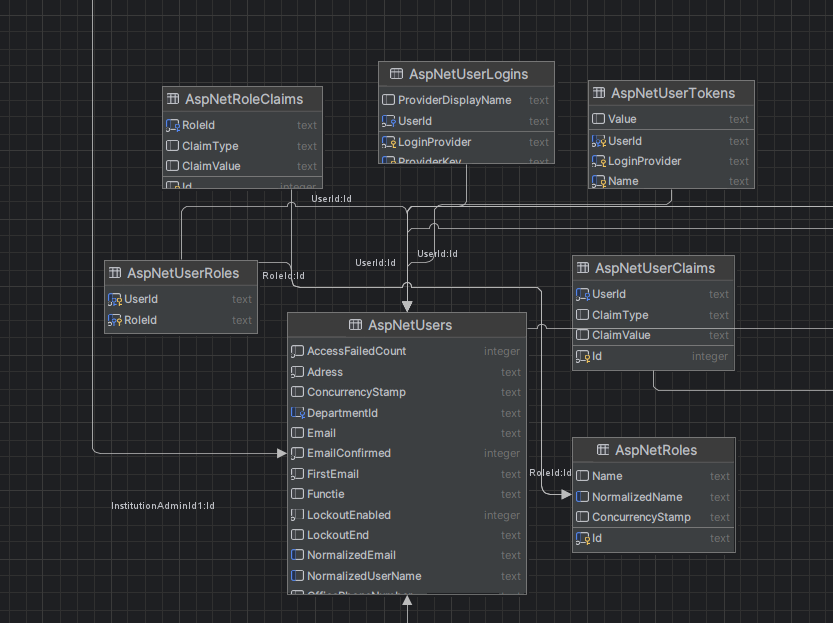
\includegraphics[width=1\textwidth]{c2/db1}
	\caption{Structura tabele autentificare si autorizare}
\end{figure}

Pentru organizarea si dezvoltarea functionalitatilor in ceea ce priviste misiunile de audit, sunt o serie de tabele care gestioneaza misiunile de audit, obiectivele acesteia, recomandarile aduse cat si documentele asociate cu respectiva misiune de audit.

\vspace{1cm}
\begin{figure}[h]
	\centering
	
	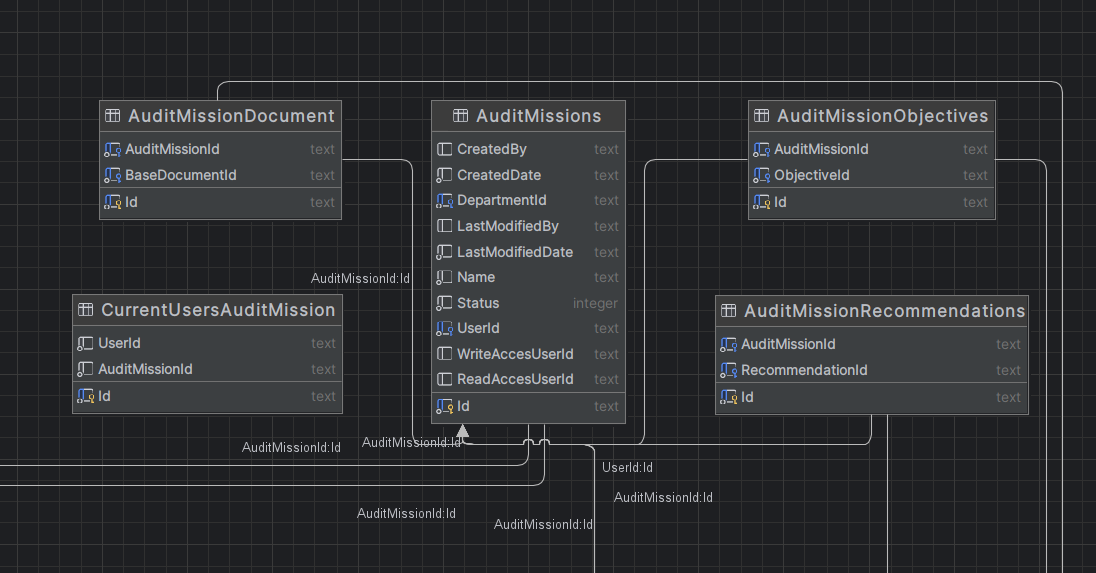
\includegraphics[width=1\textwidth]{c2/db2}
	\caption{Structura tabele gestiune misiuni de audit}
\end{figure}

\newpage
Pentru gestionarea institutiilor si a departamentelor acestora, cat si a documentelor de baza ce apartin acestora se folosec urmatoarele tabele si relatiile dintre ele.
\vspace{1cm}
\begin{figure}[h]
	\centering
	
	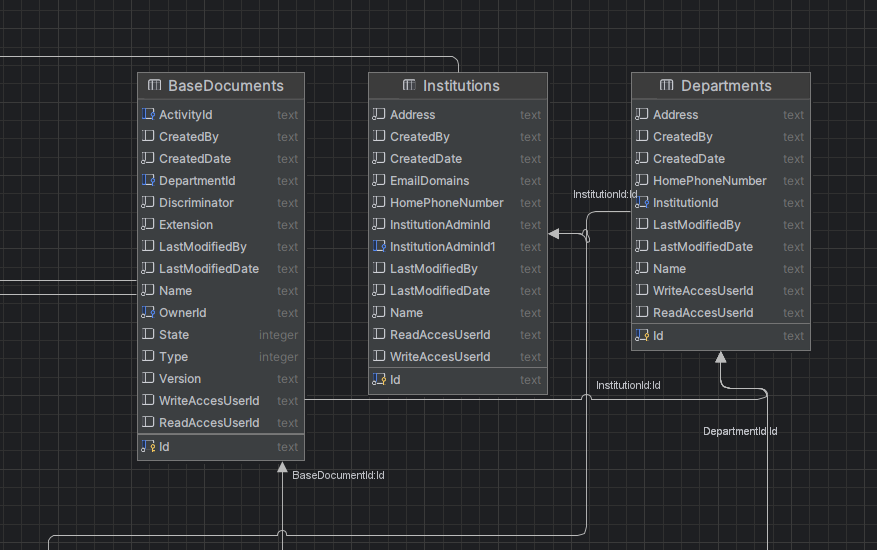
\includegraphics[width=1\textwidth]{c2/db3}
	\caption{Structura tabelelor de gestiune a institutiilor si a departamentelor}
\end{figure}

In cele din urma pentru oferirea functionalitatilor principale,cum ar fi gestionarea obiectivelor, a actiunilor acestora precum si a riscurilor si recomandarilor se utilizeaza urmatoarele tabele si relatii pe care acestea le prezinta.

\vspace{1cm}
\begin{figure}[h]
	\centering
	
	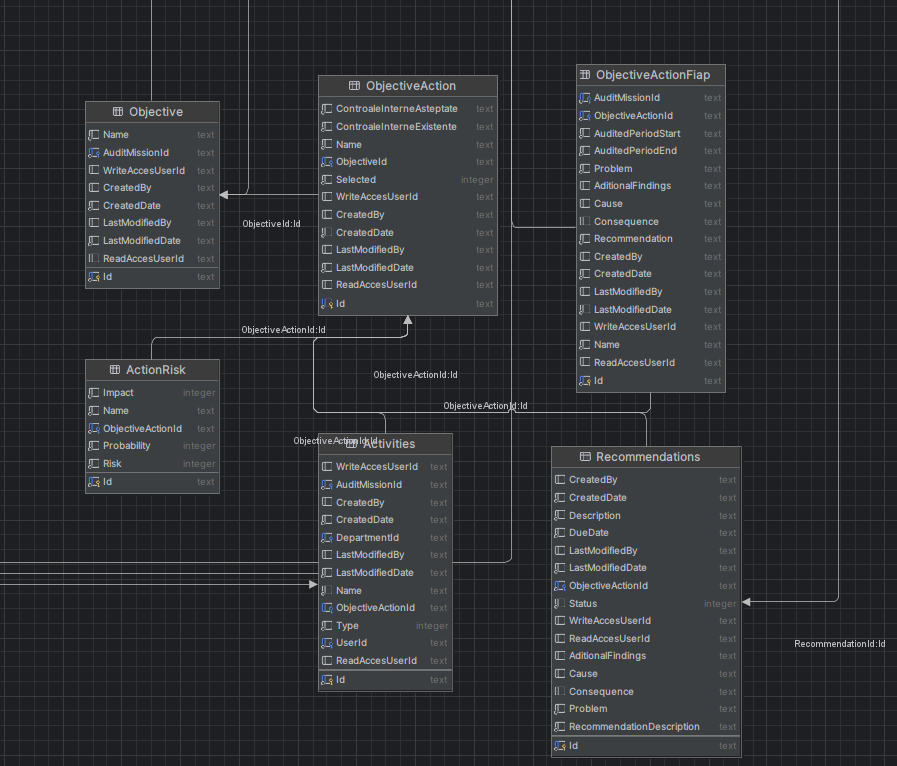
\includegraphics[width=1\textwidth]{c2/db4}
	\caption{Structura tabelelor functionalitati principale}
\end{figure}

\section{Aspecte de securitate}
Simpla dezvoltare a unei aplicatii web ce ofera utilizatorului numeroase functionalitati nu este suficienta daca aceasta aplicatie nu dispune de un set de reguli si aspecte ce  fac experienta utilizatorilor pe platforma una cat mai sigura, in care le este asigurata integritatea, confidentialitatea cat si disponibilitatea datelor si actiunilor acestora.

In dezvoltarea platformei AudIT s-a incercat utilizarea a cat mai multor standarde in ceea ce priveste securitatea actiunilor pe care un potential utilizator poate sa le faca in aplicatie, precum si a datelor si informatiilor cu care acesta lucreaza.

\subsection*{Autentificarea actiunilor}

Atat pe partea de server cat si in cea de client, sunt implementate functionalitati ce previn utilizarea \textit{endpoint-urilor} si accesarea paginilor web cand un utilizator nu este autentificat pe aplicatie. Mai mult de atat, accesul la anumite functionalitati este restrictionat doar unor categorii de utilizatori, cu un rol specific, astfel un utilizator cu rolul de reprezentant al unei institutii nu va putea accesa paginile specifice crearii si actualizarii unei misiuni de audit, intrucat rolul pe care acesta il detine nu are nivel de permisiune necesar pentru aceasta actiune.

Modalitatea prin care este verificata prin atribuirea unui \textit{token} de tip JWT (\textit{JSON web token}) fiecarui utilizator in momentul in care acesta se autentifica pe platforma, ulterior la fiecare actiune (\textit{request}) facut de acesta, fiind trimis si acest \textit{token}.\\



\textbf{Stocarea} acestui \textit{token} de acces se face intr-o maniera securizata in \textit{browser-ul} clientului sub forma unui \textit{cookie http-only}, care previne citirea acestuia de orice \textit{script} sau librarie externa din \textit{browser}, fiind utilizat doar in componenta unui \textit{request} prin HTTP, astfel protejand aplicatie si utilizatorii sai impotriva atacurilor de tip XSS(\textit{cross-site-scripting}).

\vspace{1cm}
\begin{figure}[h]
	\centering
	
	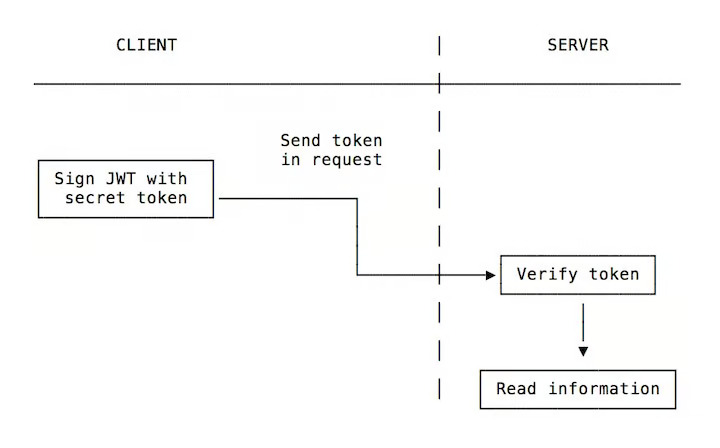
\includegraphics[width=0.7\textwidth]{c2/jwt.jpg}
	\caption{Diagrama mod functionare \textit{Web Assembly}}
\end{figure}

Pentru verificarea rolurilor si \textit{claim-urilor} pe care un utilizator le detine, este creat un \textit{endpoint} special, securizat astfel incat sa poata fi accesat doar daca in componenta \textit{request-ului} este prezent acel \textit{cookie}, care ofera informatii despre rolurile si \textit{claim-urile} specifice utilizatorului care a facut cererea. Pe baza acestora, i se permite sau i se interzice accesul la anumite pagini si actiuni pe care acesta le doreste a face.


\subsection*{Utilizarea HTTPS}

Utilizarea HTTPS atat in partea de server, cat si in cea de client impune mai multe aspecte benefice in ceea ce priveste securitatea platformei:

\begin{itemize}
	
	\item confidentialitatea datelor, https cripteaza informatia transmisa intre server si client, astfel se asigura de faptul ca sansele de interceptare si citire a  comunicatiei sunt aproape de zero;
	
	\item integritatea datelor este asigurata tot prin mecanismul de criptare a acestora, astfel asigurandu-se de faptul ca acestea ajung la destinatie neschimbate;
	
	\item autententificarea, https folosindu-se de certificate digitiale (SSL si TLS) pentru a verifica identitatea serverelor, reducand riscul unor atacuri malitioase; 
	
\end{itemize}


\subsection*{Restrictionarea inregistrarii pe platforma}

O alta modalitate prin care se mentine un nivel ridicat de securitate pe platforma o defineste restrictionarea utilizatorilor de a se inregistra pe platforma.

La pasul de creare a unui cont nou, utilizatorilor le este  impusa folosirea unei adrese de email care contine domeniul unei institutii inregistrate si configurate pe platforma. Dupa crearea cu succes a unui cont nou, acesta nu are nici o permisiune, contul fiind nevoit a fi verificat de catre o persoana cu drepturi elevate (administratorul institutiei).

Verificarea se face pe baza unui email primit de acesta in care se cere validarea identitatii noul cont creat, astfel minimizand riscul crearii a unor conturi false respectiv a unor false identitati.

\newpage
